\documentclass[tikz]{standalone}

\usepackage{tikz}

\usetikzlibrary{arrows, automata, topaths, calc, shapes.geometric}

\begin{document}


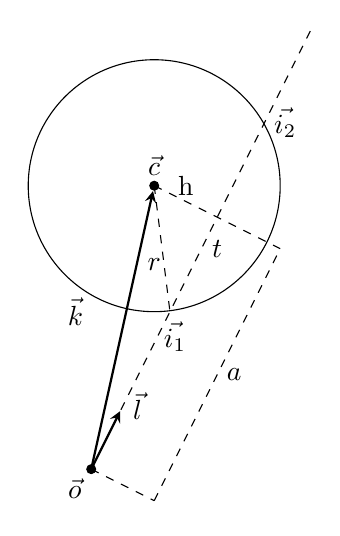
\begin{tikzpicture}[
        scale=0.4,
        important line/.style={thick},
        dashed line/.style={dashed, thin},
        pile/.style={thick, ->, >=stealth, shorten >=2pt},
        every node/.style={color=black}
    ]
    \draw[fill] (6,6) node()[above]{$\vec{c}$} circle (4pt);
    \draw (6,6) circle (4);

    \draw[fill] (4,-3) node()[below left]{$\vec{o}$} circle (4pt);

    \draw [dashed](4,-3) -- (11,11); 

    \draw [thick,pile](4,-3) -- (5,-1) node(l)[right]{$\vec{l}$};  

    \draw  (6,2) node(i1)[below right]{$\vec{i_1}$};
    \draw  (9.5,8) node(i2)[right]{$\vec{i_2}$};

    \draw [thick, pile] (4,-3) -- (6,6);
    \draw (3.5,2) node(k)[]{$\vec{k}$};

    \draw[dashed] (6,6) -- (6.5,2);
    \draw (6,3.5) node(){$r$};

    \draw[dashed] (6,6) -- (10,4);  %% (4, -2)
    \draw (7,6) node[]() {h};

    \draw[dashed] (4,-3) -- (6,-4);   %% (2,-1)

    \draw[dashed] (6,-4) -- (10,4) node()[midway, right] {$a$};

    \draw (8,4) node(){$t$};

\end{tikzpicture}    

\end{document}
